\section{Geometric Thermodynamics in Open Quantum Systems}
\label{sec:oqs}
The preceding sections established a geometric framework for
equilibrium thermodynamics based upon exact differentials of the
thermodynamic potential. Whether reconstructed from equilibrium
fluctuations, as in the Ising model, or derived analytically from
a microscopic free-energy functional, as in the spin--Peierls
model, the resulting response geometry ultimately depends upon
the existence of a thermodynamic state function. The exactness of
the free-energy differential guarantees Maxwell reciprocity,
ensures path independence, and provides the foundation for the
response manifolds developed throughout the classical theory.

Many physically important quantum systems, however, operate far
from thermodynamic equilibrium. Driven cavity-QED systems,
exciton--polariton condensates, molecular polaritons, quantum
optical devices, and nanoscale electronic systems are maintained
by a continual competition between coherent dynamics and
dissipation. Rather than relaxing toward an equilibrium Gibbs
state, these systems evolve toward nonequilibrium steady states
determined by the interplay between the system Hamiltonian and
its environment. In general, no equilibrium thermodynamic
potential exists from which the response may be obtained,
raising the natural question of whether a comparable geometric
description survives beyond equilibrium.

The answer is affirmative, although the underlying mathematical
structure changes fundamentally. Instead of an equilibrium
thermodynamic potential, the natural objects are the stationary
density operators generated by the Liouvillian dynamics. If the
externally controlled parameters evolve slowly compared with the
intrinsic relaxation timescales, the system remains close to a
continuous family of instantaneous nonequilibrium steady states.
These quasistatic trajectories provide the nonequilibrium
analogue of reversible thermodynamic processes and define a
stationary-state manifold over the space of externally controlled
parameters.

Conceptually, the progression may be summarized as
\[
H
\longrightarrow
Z
\longrightarrow
F
\longrightarrow
\text{Response Geometry},
\]
for equilibrium systems, whereas open quantum systems follow
different route:
\[
H
\longrightarrow
\mathcal{L}
\longrightarrow
\rho_{\rm ss}
\longrightarrow
\text{Response Geometry},
\]
where \(\mathcal{L}\) denotes the Liouvillian superoperator and
\(\rho_{\rm ss}\) is the nonequilibrium stationary density
operator satisfying
\[ \mathcal{L}(\bm{\lambda}) \rho_{\rm ss}(\bm{\lambda})
=0,
\]
with
\(\bm{\lambda}=(\lambda^1,\lambda^2,\ldots)\)
denoting the externally controlled parameters. The microscopic
Hamiltonian continues to determine the coherent quantum
dynamics, but the thermodynamic response is now encoded in the
parameter dependence of the stationary state rather than through
an equilibrium free-energy functional.
The absence of a global thermodynamic potential has a profound
geometric consequence. In equilibrium thermodynamics, the exact
differential \(dF\) completely determines the quasistatic work
performed along any path through the control manifold. For open
quantum systems no analogous state function generally exists.
Instead, the fundamental geometric object becomes a response
one-form defined directly on the manifold of nonequilibrium
steady states. Its exterior derivative generates a curvature
two-form whose flux governs the work performed during quasistatic
cycles, thereby extending the familiar equilibrium area laws to
driven open quantum systems.

The remainder of this section develops this quantum extension of
response geometry. We begin by constructing quasistatic
evolution on the Liouvillian control manifold and the associated
stationary-state manifold. We then introduce the quantum work
one-form and its curvature, demonstrating that quasistatic work
is governed by the flux of a curvature two-form over control
space. Finally, we show how basis misalignment between the
Hamiltonian eigenbasis and the environment-selected pointer
basis generates genuinely quantum geometric response, leading to
coherence-induced curvature, geometric cancellation of work, and
observable signatures in nonequilibrium steady states.

\subsection{Quasistatic Evolution on the Liouvillian Control Manifold}
The geometric formulation of equilibrium thermodynamics rests upon
the assumption that the system remains in equilibrium throughout
an infinitely slow thermodynamic process. At each point along a
trajectory in the control manifold, the thermodynamic state is
therefore uniquely specified by the external control parameters,
and the system evolves through a continuous sequence of
equilibrium states. This quasistatic approximation underlies the
existence of reversible thermodynamic paths and the exact
differential structure discussed in the preceding sections.

A closely analogous construction exists for open quantum systems.
Although the dynamics are intrinsically nonequilibrium, the
separation of timescales between the externally imposed control
protocol and the intrinsic relaxation dynamics allows the system
to remain arbitrarily close to an instantaneous nonequilibrium
steady state. If the control parameters vary slowly compared with
the characteristic relaxation time of the Liouvillian, the
density operator adiabatically follows the stationary solution of
the open-system dynamics. The resulting evolution defines the
nonequilibrium analogue of a reversible thermodynamic process.

Within the Markovian approximation, the reduced density operator
obeys the quantum master equation
\begin{align}
\frac{d\rho}{dt}
=
\mathcal{L}(\bm{\lambda})\rho,
\end{align}
where the Liouvillian superoperator depends parametrically upon
the externally controlled variables
\[
\bm{\lambda}
=
(\lambda^1,\lambda^2,\ldots,\lambda^N).
\]
These parameters define coordinates on a control manifold whose
points correspond to distinct physical realizations of the open
quantum system. Depending upon the physical setting,
\(\bm{\lambda}\) may include temperature, magnetic or electric
fields, chemical potentials, system--bath coupling strengths,
cavity detuning, laser amplitudes, or other experimentally
controlled quantities.

For each point on this manifold, the nonequilibrium steady state
is defined by the stationary solution
\begin{align}
\mathcal{L}(\bm{\lambda})
\rho_{\rm ss}(\bm{\lambda})
=
0,
\end{align}
subject to the normalization condition
\[
\mathrm{Tr}
\left[
\rho_{\rm ss}
\right]
=
1.
\]
Provided the control parameters evolve sufficiently slowly, the
density operator remains close to the instantaneous stationary
state,
\begin{align}
\rho(t)
\simeq
\rho_{\rm ss}
\!\left(
\bm{\lambda}(t)
\right),
\end{align}
so that the physical evolution is completely characterized by a
trajectory through the manifold of stationary density operators.
The dynamics therefore reduce to geometry on the control
manifold, in direct analogy with quasistatic evolution in
equilibrium thermodynamics.

Throughout this review, we shall therefore use the term quasistatic reversible process to denote transport for which the externally controlled parameters evolve sufficiently slowly that the system remains on the manifold of instantaneous stationary states. Although entropy may continue to be exchanged with the environment, no additional irreversibility is introduced by the driving protocol itself. This definition provides the natural nonequilibrium extension of the reversible quasistatic processes of equilibrium thermodynamics.

This viewpoint provides the conceptual bridge between classical
and quantum response geometry. In equilibrium, quasistatic
trajectories are generated by an exact thermodynamic potential.
In open quantum systems, they are generated instead by the family
of stationary density operators determined by the Liouvillian.
The geometric description therefore shifts from a manifold of
equilibrium states to a manifold of nonequilibrium steady states,
while preserving the fundamental notion of quasistatic transport
through control space.
Having established the kinematics of quasistatic evolution, we
next seek the appropriate analogue of the equilibrium
differential \(dF\). As we shall show, the absence of a global
thermodynamic potential naturally leads to the introduction of a
response one-form whose non-exactness gives rise to an intrinsic
geometric curvature.


\subsection{Quantum Work and Heat Along Quasistatic Trajectories}
Having established the notion of quasistatic evolution on the
Liouvillian control manifold, we now seek the nonequilibrium
analogue of the First Law of thermodynamics. The central question
is not whether work and heat remain meaningful for open quantum
systems, but rather how these quantities are expressed in terms
of the stationary density operator and the externally controlled
Hamiltonian.
For a system described by the instantaneous nonequilibrium steady
state \(\rho_{\rm ss}(\bm{\lambda})\), the internal energy is
naturally defined as the expectation value of the Hamiltonian,
\begin{align}
U(\bm{\lambda})
=
\mathrm{Tr}
\left[
\rho_{\rm ss}(\bm{\lambda})
H(\bm{\lambda})
\right].
\end{align}
The total differential of the internal energy is therefore
\begin{align}
dU
=
d\,
\mathrm{Tr}
(\rho H)
=
\mathrm{Tr}
(H\,d\rho)
+
\mathrm{Tr}
(\rho\,dH),
\end{align}
where we have omitted the explicit parameter dependence for
clarity. This decomposition is completely general and follows
solely from the product rule for differentiation.
The two contributions possess an immediate thermodynamic
interpretation. The first term describes changes in the quantum
state while the Hamiltonian is held fixed and therefore
represents energy exchanged between the system and its
environment. We identify this contribution as the quasistatic
heat,
\begin{align}
\delta Q
=
\mathrm{Tr}
(H\,d\rho).
\end{align}
The second term describes changes in the Hamiltonian generated by
variations of the external control parameters while the
instantaneous stationary state is held fixed. This contribution
corresponds to the quasistatic work,
\begin{align}
\delta W
=
\mathrm{Tr}
(\rho\,dH).
\end{align}
Consequently, the First Law retains its familiar form,
\begin{align}
dU
=
\delta Q
+
\delta W.
\end{align}
The important distinction from equilibrium thermodynamics is that
neither \(\delta Q\) nor \(\delta W\) is, in general, an exact
differential. Although the internal energy remains a state
function, the work and heat exchanged during transport through
the Liouvillian control manifold depend upon the path followed by
the external control parameters. 
%
%The transition from equilibrium
%to nonequilibrium thermodynamics is therefore not the loss of the
%First Law, but the loss of integrability.
%

\begin{tcolorbox}[
enhanced,
colback=gray!8,
colframe=black,
boxrule=0.8pt,
arc=2mm,
left=2mm,
right=2mm,
top=1.5mm,
bottom=1.5mm]
\centering
\itshape
The transition from equilibrium to nonequilibrium
thermodynamics is not the loss of the First Law,
but the loss of integrability.
\end{tcolorbox}

The internal energy remains a well-defined state function satisfying the First Law. What changes is the mathematical character of the work and heat differentials. In equilibrium they derive from an exact differential and are therefore path independent. In nonequilibrium steady states, the quasistatic work is described by a generally non-exact one-form, so that transport around closed cycles can accumulate finite geometric work. It is this loss of integrability—not the failure of energy conservation—that gives rise to the response geometry developed throughout the remainder of this section.

To expose the geometric structure of the work, we write the
Hamiltonian differential as
\begin{align}
dH
=
\sum_\mu
\frac{\partial H}
{\partial\lambda^\mu}
d\lambda^\mu,
\end{align}
where the \(\lambda^\mu\) are coordinates on the control
manifold. Substituting this expression into the work differential
gives
\begin{align}
\delta W
&=
\sum_\mu
\mathrm{Tr}
\left[
\rho_{\rm ss}
\frac{\partial H}
{\partial\lambda^\mu}
\right]
d\lambda^\mu
\\
&\equiv
A_\mu(\bm{\lambda})
\,d\lambda^\mu,
\end{align}
where
\begin{align}
A_\mu(\bm{\lambda})
=
\mathrm{Tr}
\left[
\rho_{\rm ss}(\bm{\lambda})
\frac{\partial H}
{\partial\lambda^\mu}
\right]
\end{align}
defines the components of the quantum work one-form.
Unlike the equilibrium differential \(dF\), the one-form
\(A_\mu d\lambda^\mu\) is generally not exact. 

Consequently, the
quasistatic work performed between two points of the control
manifold depends upon the trajectory connecting them. This
non-integrability is the origin of the geometric structure that
distinguishes nonequilibrium steady states from their equilibrium
counterparts. In the following subsection we show that the
exterior derivative of the work one-form defines a curvature
two-form whose flux governs the work accumulated during
quasistatic cyclic processes.



\subsection{Local Response Tensor and Geometric Decomposition}
The work one-form introduced in the preceding section provides
the natural differential description of quasistatic work in open
quantum systems. While its line integral determines the work
performed along a particular thermodynamic path, the local
geometry of the response manifold is encoded in its derivatives.

In this sense, the work one-form plays a role analogous to a
vector potential in gauge theory: it is the generating object
from which the intrinsic local geometry is constructed.
We therefore introduce the local response tensor
\begin{align}
\chi_{\mu\nu}
=
\frac{\partial A_\mu}
{\partial\lambda^\nu},
\end{align}
which characterizes the differential response of the system to
infinitesimal changes of the external control parameters.

Unlike equilibrium thermodynamics, where the response matrix is
necessarily symmetric owing to the exactness of the free-energy
differential, the nonequilibrium response tensor generally
contains both reciprocal and nonreciprocal components.
The response tensor admits the unique decomposition
\begin{align}
\chi_{\mu\nu}
=
G_{\mu\nu}
+
F_{\mu\nu},
\end{align}
where
\begin{align}
G_{\mu\nu}
=
\frac{1}{2}
\left(
\chi_{\mu\nu}
+
\chi_{\nu\mu}
\right)
\end{align}
is the symmetric response metric, while
\begin{align}
F_{\mu\nu}
=
\frac{1}{2}
\left(
\chi_{\mu\nu}
-
\chi_{\nu\mu}
\right)
\end{align}
is the antisymmetric response curvature.
This decomposition generalizes the familiar equilibrium response
matrix. In equilibrium, the existence of an exact thermodynamic
potential requires the mixed derivatives to commute, so that
\[
F_{\mu\nu}=0,
\]
and the response is completely characterized by the symmetric
metric tensor. Nonequilibrium steady states remove this
integrability constraint, permitting a finite antisymmetric
sector that encodes the nonreciprocal response generated by
coherence and dissipation.

The physical interpretation of the two tensors is
complementary. The symmetric metric characterizes local
susceptibilities, reciprocal response, fluctuations, and the
stability of the stationary state. The antisymmetric curvature
measures the failure of reciprocity, determines the geometric
contribution to quasistatic work, and governs the holonomy
associated with transport around closed loops in parameter space.

This decomposition establishes a direct correspondence between
equilibrium and nonequilibrium response geometry. Equilibrium
thermodynamics is recovered as the special case for which the
response tensor is purely symmetric, while open quantum systems
possess a richer local geometry consisting of both metric and
curvature fields. The work one-form therefore serves primarily
as the generating potential for these local geometric objects
rather than as the fundamental object of the theory itself.

An important consequence of this formulation is that local
fluctuations about the nonequilibrium steady state naturally
probe the response geometry. Just as equilibrium covariance
matrices provide the microscopic origin of thermodynamic
metrics, fluctuations of observables about
\(\rho_{\rm ss}\) characterize the local response of the
stationary state. This observation forms the basis for the
response reconstruction framework developed in the following
section and provides the conceptual bridge between response
geometry and information-geometric approaches based upon the
Bures and quantum Fisher metrics.


\subsection{The Gibbs Manifold as the Integrable Limit}
Before considering nonequilibrium steady states, it is
instructive to examine the special case in which the
stationary density operator is the canonical Gibbs state.
This establishes the equilibrium limit of the response
geometry and identifies the condition under which the
antisymmetric response necessarily vanishes.

Suppose the stationary state is given by
\begin{align}
\rho_{\rm G}(\bm{\lambda})
=
\frac{e^{-\beta H(\bm{\lambda})}}
{Z(\bm{\lambda})},
\end{align}
with partition function
\begin{align}
Z(\bm{\lambda})
=
{\rm Tr}
\left[
e^{-\beta H(\bm{\lambda})}
\right],
\end{align}
and Helmholtz free energy
\begin{align}
F(\bm{\lambda})
=
-k_{\rm B}T
\ln Z(\bm{\lambda}).
\end{align}
The generalized forces follow from the equilibrium
thermodynamic potential,
\begin{align}
A_\mu
=
-\frac{\partial F}
{\partial\lambda^\mu},
\end{align}
where the sign convention depends upon the definition of
the generalized work variables. Differentiating once more
gives the local response tensor,
\begin{align}
\chi_{\mu\nu}
=
\frac{\partial A_\mu}
{\partial\lambda^\nu}
=
-
\frac{\partial^2F}
{\partial\lambda^\mu
 \partial\lambda^\nu}.
\end{align}
Since the free energy is a thermodynamic state function,
its mixed derivatives commute,
\begin{align}
\frac{\partial^2F}
{\partial\lambda^\mu
 \partial\lambda^\nu}
=
\frac{\partial^2F}
{\partial\lambda^\nu
 \partial\lambda^\mu},
\end{align}
so that
\begin{align}
\chi_{\mu\nu}
=
\chi_{\nu\mu}.
\end{align}
The antisymmetric sector therefore vanishes identically,
\begin{align}
F_{\mu\nu}
=
\frac12
\left(
\chi_{\mu\nu}
-
\chi_{\nu\mu}
\right)
=
0.
\end{align}
Thus, every Gibbs equilibrium state generates a purely
metric response manifold. Reciprocity is guaranteed by
the existence of the equilibrium thermodynamic
potential, and the response geometry is completely
described by the symmetric response tensor.

This observation provides a simple criterion for
identifying genuinely nonequilibrium response.
Whenever the stationary state may be written as
\begin{align}
\rho_{\rm ss}
\propto
e^{-\beta H},
\end{align}
the response remains integrable and the antisymmetric
sector vanishes. Consequently, the appearance of a
finite antisymmetric response is not a generic quantum
effect but a signature that the stationary state can no
longer be represented by a global Gibbs distribution.

The central question therefore becomes:
\emph{what physical mechanism drives the stationary
state away from the Gibbs manifold?}
For open quantum systems the answer is the competition
between coherent Hamiltonian evolution and
environmentally induced decoherence. The simplest
realization of this competition is provided by a driven
qubit whose pointer basis does not coincide with the
Hamiltonian eigenbasis. This example provides the
minimal setting in which the transition from equilibrium
response to genuinely nonequilibrium response can be
studied explicitly.

\subsection{A Bloch-Sphere Illustration of Nonequilibrium Response Geometry}
The abstract construction developed in the preceding sections is
most easily illustrated using the simplest nontrivial open
quantum system---a driven two-level system. Despite its apparent
simplicity, the qubit captures all of the essential ingredients
required for nonequilibrium response geometry, including coherent
dynamics, environmental decoherence, basis complementarity, and
the emergence of both reciprocal and nonreciprocal response.

Moreover, because the stationary state admits a geometric
representation on the Bloch sphere, the resulting response
geometry can be visualized directly.
We consider a qubit described by the Hamiltonian
\begin{align}
H(\omega,g)
=
\frac{\omega}{2}\sigma_z
+
\frac{g}{2}\sigma_x,
\end{align}
where the control parameters
\begin{align}
\bm{\lambda}
=
(\omega,g,T)
\end{align}
consist of the level splitting, transverse coupling, and bath
temperature. The qubit is coupled weakly to a Markovian
environment so that its reduced dynamics are governed by a
Lindblad master equation
\begin{align}
\frac{d\rho}{dt}
=
-i[H,\rho]
+
\mathcal{D}[\rho],
\end{align}
where the dissipator $\mathcal{D}$ describes energy relaxation
and dephasing induced by the surrounding bath. For fixed values
of the control parameters, the nonequilibrium steady state
satisfies
\begin{align}
\mathcal{L}(\bm{\lambda})
\rho_{\rm ss}
=
0.
\end{align}
The corresponding stationary density matrix may be represented in
Bloch form,
\begin{align}
\rho_{\rm ss}
=
\frac{1}{2}
\left(
I
+
\mathbf{r}\cdot\boldsymbol{\sigma}
\right),
\end{align}
where $\mathbf r=(r_x,r_y,r_z)$ is the stationary Bloch vector.
The entire thermodynamic response of the qubit is therefore
encoded in the evolution of the Bloch vector over the control
manifold $(\omega,g,T)$.

The equilibrium limit provides an important reference point. When
the dissipative dynamics thermalize the system in the
Hamiltonian eigenbasis, the stationary state reduces to the Gibbs
state,
\begin{align}
\rho_{\rm ss}
=
\rho_{\rm Gibbs}
=
\frac{e^{-\beta H}}
{\mathrm{Tr}(e^{-\beta H})},
\end{align}
for which the Bloch vector is aligned with the effective magnetic
field defined by the Hamiltonian. In this limit the work one-form
is integrable, the response tensor is symmetric, and the
antisymmetric response vanishes, reproducing the equilibrium
geometry discussed in the preceding sections.

More generally, however, the environment need not select the
Hamiltonian eigenbasis as its preferred basis. Instead, the
dissipative dynamics define a pointer basis that may be rotated
with respect to the instantaneous energy eigenstates. The
stationary density matrix is then no longer diagonal in the
Hamiltonian basis and acquires steady-state coherences. The
nonequilibrium steady state is therefore determined by the
competition between coherent Hamiltonian evolution and
environmentally induced basis selection rather than by the
Hamiltonian alone.

This basis mismatch provides the minimal physical mechanism for
the emergence of nonequilibrium response geometry. As the pointer
basis rotates away from the Hamiltonian eigenbasis, the local
response tensor acquires an antisymmetric component, signaling
the breakdown of equilibrium reciprocity. The qubit therefore
provides the simplest realization of the transition from an
integrable equilibrium response manifold to the richer response
geometry characteristic of driven nonequilibrium steady states.
This example also introduces a broader conceptual theme that
reappears throughout the remainder of this review. The geometry
of an open quantum system is not determined solely by its
Hamiltonian or solely by its environment, but by the
complementarity between coherent dynamics, environmental basis
selection, and the observational basis used to interrogate the
system. In later sections we formalize this relationship as the
complementarity--preparation--environment (CPE) triality and show
that it provides a unifying framework for understanding response
geometry, information geometry, and spectroscopic
reconstruction.

\subsection{Response Immersion and K\"ahler Compatibility}
\label{sec:KahlerCompatibility}
One of the central themes of this review is that reciprocal and
nonreciprocal response should not be viewed as unrelated physical
phenomena. The response metric and response curvature arise from
the same underlying stationary state and describe complementary
aspects of how that state changes under variations of the external
controls. This observation naturally raises a geometric question:
are these two tensors fundamentally independent, or do they admit
a common geometric origin?

For a two-dimensional control manifold, this question admits a
remarkably simple answer. Suppose that the response of the system
may be represented locally by a smooth response map
%
\begin{equation}
\Phi:
(\lambda^1,\lambda^2)
\longrightarrow
\mathbb{R}^2,
\end{equation}
%
whose components encode the local response of the stationary
state. The reciprocal response metric is then obtained as the
pullback of the Euclidean metric,
%
\begin{equation}
G_{\mu\nu}
=
\partial_\mu\Phi\cdot
\partial_\nu\Phi,
\end{equation}
%
while the antisymmetric response curvature is obtained from the
oriented area swept out by the same response map,
%
\begin{equation}
F_{12}
=
\det(D\Phi),
\end{equation}
%
where $D\Phi$ denotes the Jacobian of the immersion.

The remarkable observation is that these quantities are not
independent. Since
%
\begin{equation}
G=(D\Phi)^T(D\Phi),
\end{equation}
%
one immediately finds
%
\begin{equation}
\det G
=
\det\!\left[(D\Phi)^T(D\Phi)\right]
=
(\det D\Phi)^2.
\end{equation}
%
Because the curvature is precisely the Jacobian determinant of the
same immersion,
%
\begin{equation}
F_{12}
=
\det(D\Phi),
\end{equation}
%
it follows that
%
\begin{equation}
\boxed{
\det G
=
F_{12}^{\,2}.
}
\label{eq:ResponseImmersionIdentity}
\end{equation}
Equation~(\ref{eq:ResponseImmersionIdentity}) is the Response
Immersion Theorem. It establishes that whenever the reciprocal
response metric and the antisymmetric response curvature arise
from the same underlying response map, they satisfy an exact
compatibility relation. The response geometry therefore possesses
far more internal structure than is apparent from either tensor
alone.

An immediate consequence is obtained by introducing the operator
%
\begin{equation}
J
=
G^{-1}F.
\end{equation}
%
For a two-dimensional response manifold,
Eq.~(\ref{eq:ResponseImmersionIdentity}) implies
%
\begin{equation}
J^2=-I,
\end{equation}
%
showing that the metric and curvature define a compatible
almost-complex structure. In the language of differential
geometry, the induced response manifold is therefore K\"ahler.
The significance of this result is primarily physical rather than
mathematical. K\"ahler geometry appears throughout mathematical
physics because it unifies notions of distance, orientation, and
symplectic transport within a single geometric framework. Here the
same structure emerges naturally from response theory itself. The
response metric measures reciprocal susceptibility and
distinguishability, while the response curvature measures cyclic
transport and geometric work. The Response Immersion Theorem shows
that these quantities need not be regarded as independent
descriptors of the dynamics; rather, they may represent
complementary projections of a single underlying response
geometry.

This interpretation also clarifies the role of the two-level
system discussed throughout this review. The theorem is local: it
depends only on the existence of a two-dimensional response chart.
Consequently, the canonical two-level system should not be viewed
merely as a simple physical model, but as the universal local
coordinate chart for response geometry. More complicated open
quantum systems introduce additional response coordinates and
higher-dimensional control manifolds, yet their local geometric
structure is frequently governed by the effective coupling of
pairs of pathways. The two-level system therefore plays the same
role in response geometry that the tangent plane plays in
classical differential geometry---it provides the canonical local
description from which the geometry of more complicated systems is
constructed.

%============================================================
% Callout Box: Response Immersion Theorem
%============================================================
\begin{tcolorbox}[
colback=blue!3,
colframe=blue!60!black,
title=\textbf{Response Immersion Theorem: Why It Matters},
fonttitle=\bfseries]
A central result of this work is that the reciprocal response metric
$G_{\mu\nu}$ and the antisymmetric response curvature
$F_{\mu\nu}$ need not be regarded as independent geometric objects.
Whenever both arise from the same underlying response immersion,
they satisfy the exact identity
\begin{equation}
\boxed{
\det G = F_{12}^{\,2}.
}
\end{equation}
This relation has an important physical consequence.  The metric,
which characterizes reciprocal susceptibility and
distinguishability, and the curvature, which characterizes cyclic
transport and geometric work, become complementary projections of
the same underlying response geometry rather than unrelated
quantities.
Equivalently, the response operator
\[
J = G^{-1}F
\]
defines a compatible complex structure satisfying
\[
J^2=-I,
\]
so that the local response manifold possesses a K\"ahler geometry.
Thus, the appearance of K\"ahler structure is not imposed as an
additional mathematical assumption, but emerges naturally whenever
the reciprocal and nonreciprocal sectors of response share a common
geometric origin.
The theorem therefore provides a unifying geometric interpretation
of response theory: \emph{reciprocal response determines local
distance, nonreciprocal response determines local circulation, and
together they define the intrinsic geometry of the response
manifold.}
\end{tcolorbox}


\subsection{Response Geometry versus Information Geometry}
The decomposition of the local response tensor into symmetric
and antisymmetric components immediately raises an important
question: how does response geometry relate to the information
geometry of quantum states? Both constructions assign geometric
objects to the same family of stationary density operators, yet
they arise from fundamentally different physical principles.
The response tensor introduced above is constructed from the
change in observable expectation values under infinitesimal
variations of the external control parameters. Its symmetric
component,
\begin{align}
G_{\mu\nu}
=
\frac12
\left(
\chi_{\mu\nu}
+
\chi_{\nu\mu}
\right),
\end{align}
measures reciprocal response, while its antisymmetric component,
\begin{align}
F_{\mu\nu}
=
\frac12
\left(
\chi_{\mu\nu}
-
\chi_{\nu\mu}
\right),
\end{align}
governs nonreciprocal response and geometric work during
quasistatic cycles.
By contrast, the Bures metric
\begin{align}
g^{\rm B}_{\mu\nu}
=
\frac14
\left[
\partial_\mu\mathbf r\cdot\partial_\nu\mathbf r
+
\frac{
(\mathbf r\cdot\partial_\mu\mathbf r)
(\mathbf r\cdot\partial_\nu\mathbf r)
}
{1-|\mathbf r|^2}
\right],
\end{align}
is an information-geometric object. It measures the
distinguishability of neighboring quantum states and is
proportional to the quantum Fisher information. Unlike the
response tensor, it contains no antisymmetric component and
therefore cannot describe geometric work or nonreciprocal
response.

\begin{figure*}[t]
\centering
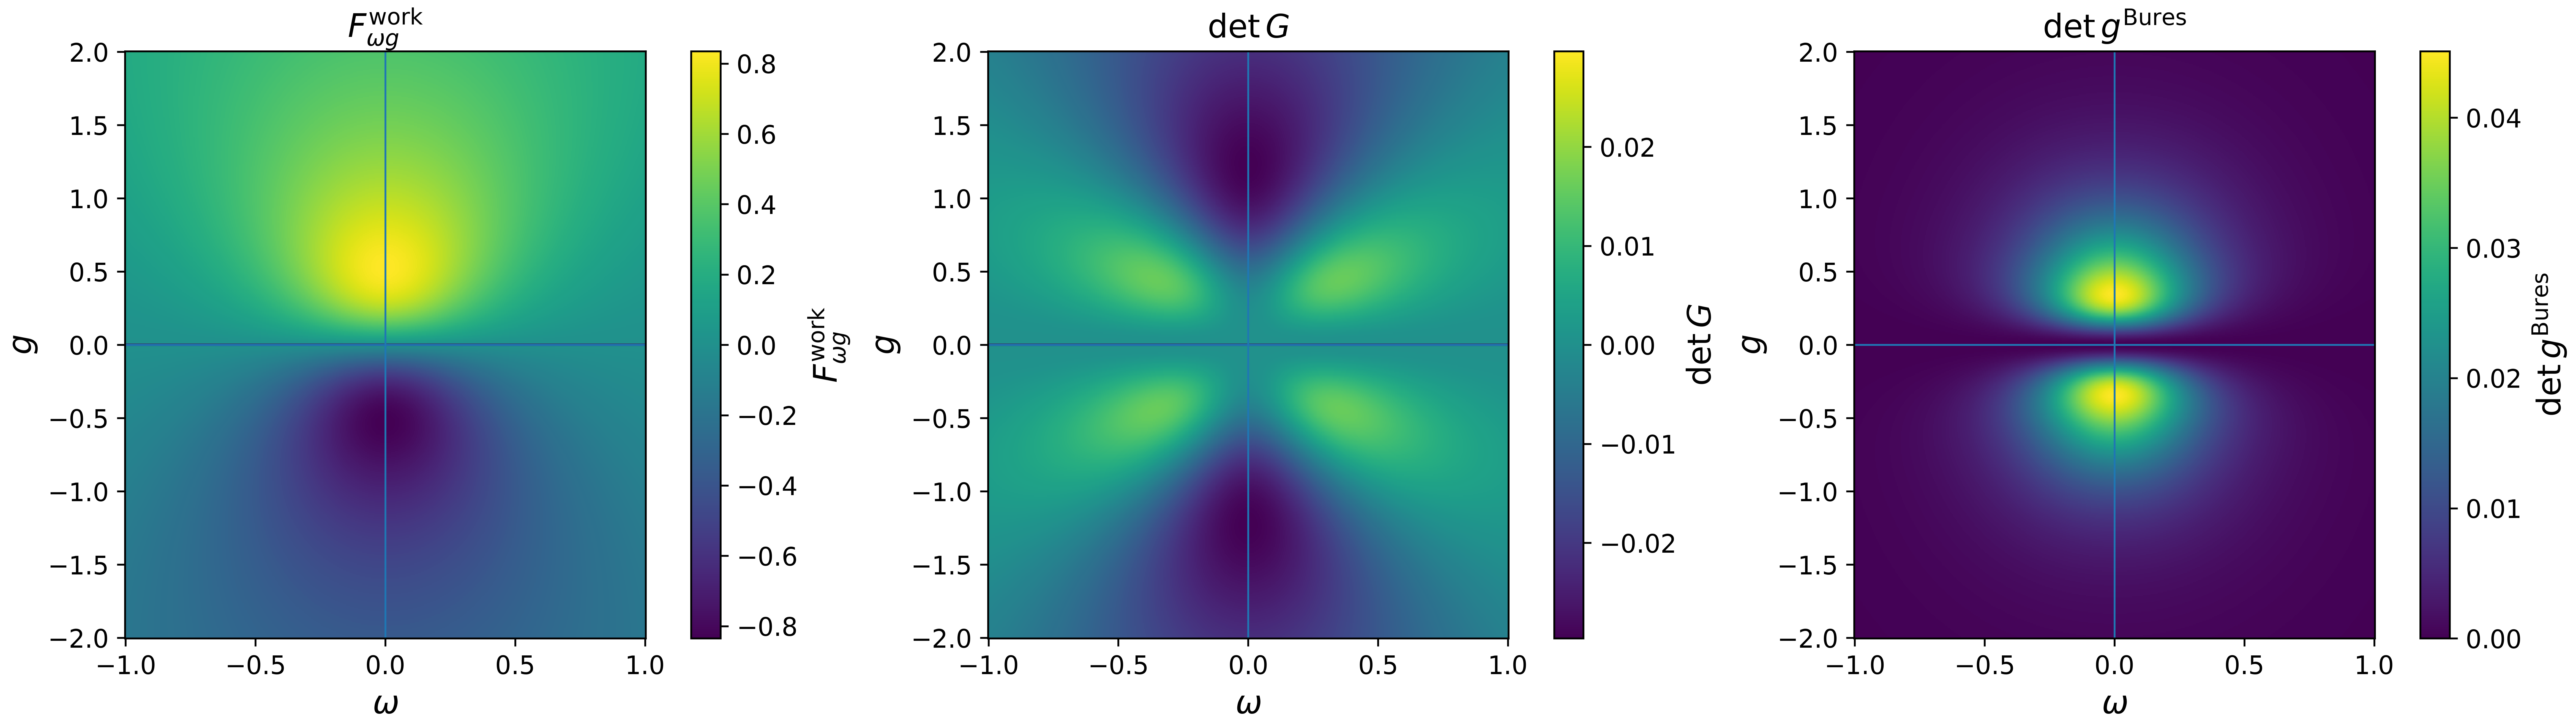
\includegraphics[width=\textwidth]{Figures/Figure1_F_vs_G_vs_g.png}
\caption{
\textbf{Comparison of response geometry and information geometry for a driven open quantum system.}
The three panels display complementary geometric structures
defined over the same two-dimensional control manifold
parameterized by the Hamiltonian frequency $\omega$ and coherent
coupling strength $g$. All quantities are computed from the same
family of nonequilibrium stationary density operators of the
driven qubit model.
(a) Antisymmetric work curvature
$F_{\omega g}^{\rm work}$.
This field governs the geometric contribution to quasistatic
cyclic work and changes sign under reversal of the orientation of
the control cycle. The nodal line separates regions of opposite
geometric orientation and is analogous to the curvature fields
introduced earlier for equilibrium thermodynamic systems.
(b) Determinant of the symmetric response metric,
$\det G$.
This quantity measures the magnitude of the reciprocal component
of the local response tensor and characterizes the local
susceptibility of the nonequilibrium steady state to changes in
the external control parameters. Unlike the antisymmetric
curvature, the response metric is insensitive to the orientation
of parameter-space loops.
(c) Determinant of the Bures metric,
$\det g^{\rm Bures}$.
The Bures metric is an information-geometric measure of the
distinguishability of neighboring stationary density operators
and is proportional to the quantum Fisher information. It
contains no antisymmetric component and therefore cannot describe
geometric work or nonreciprocal response.
Although all three fields are generated from the same family of
stationary states, they exhibit markedly different spatial
organization. The work curvature possesses a signed dipolar
structure associated with nonreciprocal response, the response
metric develops a quadrupolar pattern characteristic of
reciprocal susceptibility, and the Bures metric is localized near
the avoided crossing where neighboring stationary states become
most rapidly distinguishable. Their coexistence demonstrates that
nonequilibrium quantum systems possess multiple, complementary
geometric structures. Response geometry and information geometry
are therefore related through the common stationary-state
manifold, but they encode fundamentally different physical
properties.
}
\label{fig:F_G_Bures}
\end{figure*}

Figure~\ref{fig:F_G_Bures} compares these geometric structures
for the driven qubit introduced in the previous subsection.
Panel (a) shows the antisymmetric work curvature
$F_{\omega g}^{\rm work}$, panel (b) the determinant of the
symmetric response metric $G$, and panel (c) the determinant of
the Bures metric. All three quantities are evaluated on the same
control manifold and are generated from the same family of
nonequilibrium steady states.
Several observations immediately emerge. First, the
antisymmetric work curvature possesses a signed dipolar
structure reflecting the orientation dependence of quasistatic
cycles. Second, the response metric exhibits a quadrupolar
organization associated with reciprocal susceptibility. Finally,
the Bures metric is concentrated near the avoided crossing,
where neighboring stationary states become most rapidly
distinguishable. Although all three fields derive from the same
steady-state manifold, they emphasize fundamentally different
aspects of the response.
This comparison demonstrates that response geometry and
information geometry are complementary rather than equivalent.
The response metric characterizes how physical observables change
under external driving, whereas the Bures metric characterizes
how rapidly the quantum state itself changes. Agreement between
the two is therefore neither expected nor required. Instead,
their differences provide additional physical information about
the relationship between dynamical response and state-space
structure.
This distinction motivates the introduction of an enlarged
response tensor whose Hermitian structure naturally contains both
the reciprocal response metric and the antisymmetric work
curvature. Information geometry then appears not as a
replacement for response geometry, but as an independent metric
structure defined on the same manifold of stationary states.




\subsection{Complementarity and the Triality Manifold}
The Bloch representation introduced in the preceding
subsection provides a convenient description of the
stationary state of a driven qubit. While the Cartesian
coordinates $(x,y,z)$ completely specify the reduced
density operator, they do not directly distinguish the
different physical resources that characterize an open
quantum system. It is therefore useful to introduce a
coordinate system whose components possess immediate
physical interpretation.

For a stationary Bloch vector
\begin{align}
\mathbf{r}
=
(x,y,z),
\end{align}
we define the coherence
\begin{align}
C
=
\sqrt{x^2+y^2},
\end{align}
which measures the magnitude of the off-diagonal
coherence within the pointer-basis plane, together with
the predictability
\begin{align}
P
=
z,
\end{align}
which measures the population imbalance between the
pointer states. The Bloch-vector magnitude is
\begin{align}
R
=
\sqrt{x^2+y^2+z^2},
\end{align}
with $R\le1$, where equality holds only for pure states.

The departure from the Bloch-sphere surface is measured
by the openness coordinate
\begin{align}
E
=
\sqrt{1-R^2},
\end{align}
which quantifies the contraction of the Bloch sphere
resulting from environmental mixing and reduction from
the larger system--environment Hilbert space.

These variables satisfy the normalized triality relation
\begin{align}
C^2+P^2+E^2=1,
\label{eq:triality}
\end{align}
which defines a quarter-sphere manifold containing all
physically admissible reduced steady states. In this
representation, coherence and predictability specify the
cylindrical projection of the Bloch vector, while
openness appears naturally as a radial deficit. Pure
states lie on the boundary $E=0$, whereas increasing
interaction with the environment moves the system
toward the interior of the manifold.

\begin{figure*}[t]
\centering
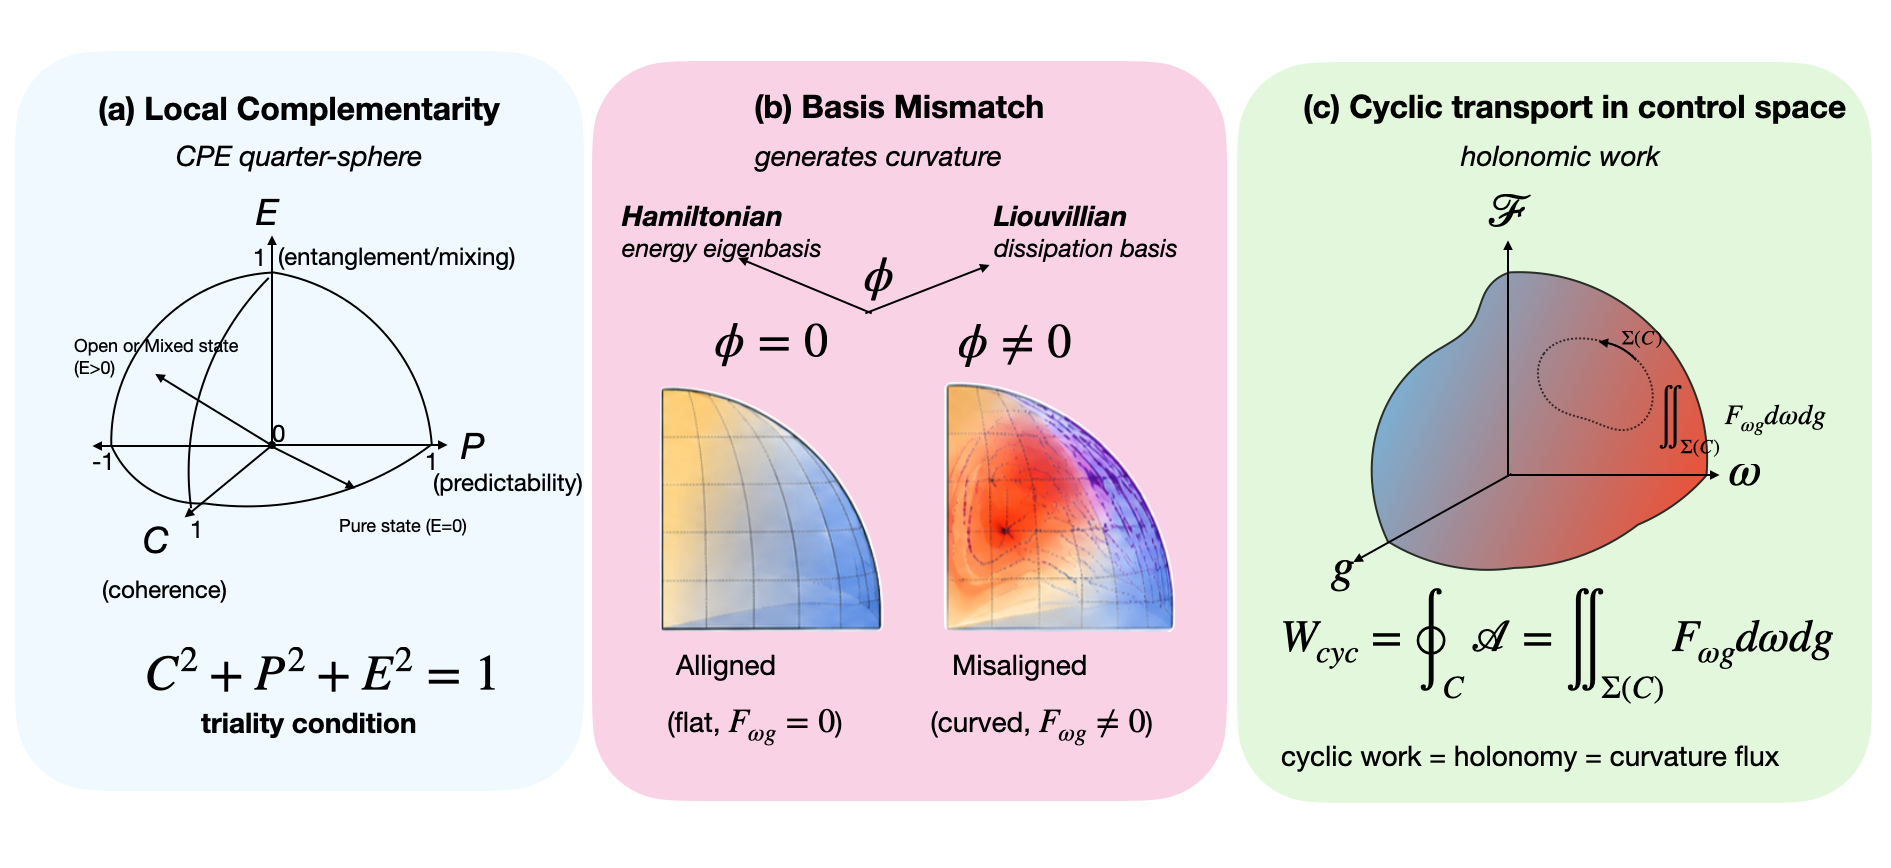
\includegraphics[width=\textwidth]{Figures/CPE_Fig0.png}
\caption{
\textbf{Complementarity and the triality manifold for open quantum systems.}
(a) The complementarity variables coherence $C$,
predictability $P$, and openness $E$ provide a natural
coordinate system for the reduced steady-state manifold of
a driven qubit. These variables satisfy the normalized
triality relation
$C^{2}+P^{2}+E^{2}=1$,
so that every physically admissible reduced state occupies
a point on the quarter sphere. Coherence measures the
off-diagonal quantum superposition within the pointer-basis
plane, predictability measures the population imbalance,
and openness quantifies the contraction of the Bloch sphere
resulting from environmental mixing.
(b) Schematic illustration of the competition between
coherent Hamiltonian evolution and environmentally selected
pointer states. When the Hamiltonian and pointer bases are
aligned, the stationary state reduces to the Gibbs manifold
and the response is integrable. Misalignment between these
structures produces genuinely nonequilibrium steady states
whose response cannot, in general, be derived from a global
thermodynamic potential.
(c) Conceptual representation of quasistatic transport over
the control manifold. Cyclic evolution generates a geometric
response that depends upon the path taken through parameter
space rather than only the initial and final states. The
formal relationship between the local response tensor, the
antisymmetric response field, and the resulting cyclic work
is developed in the following sections.
Throughout this review, the triality manifold serves as the
canonical state-space representation for open quantum
systems. The complementarity variables $(C,P,E)$ specify
the local steady state, while subsequent figures paint
response fields onto this manifold to illustrate the
relationship between complementarity, nonequilibrium
response, geometric transport, and observational
reconstruction.
}
\label{fig:CPE}
\end{figure*}

Figure~\ref{fig:CPE} summarizes this geometric
construction. Panel (a) illustrates the triality
manifold defined by Eq.~(\ref{eq:triality}), where every
point corresponds to a physically admissible reduced
steady state. The variables $(C,P,E)$ therefore provide
a physically motivated coordinate system whose axes
represent coherence, predictability, and openness,
respectively, rather than Cartesian components of the
Bloch vector.


The remaining panels anticipate the geometric structure
developed in the following sections. Panel (b)
illustrates how complementarity between coherent
Hamiltonian evolution and environmentally selected
pointer states generates nontrivial response on the
triality manifold, while panel (c) depicts the cyclic
transport associated with quasistatic evolution over the
control manifold. At this stage these panels should be
viewed primarily as a roadmap for the subsequent
development. Their physical interpretation in terms of
response geometry, antisymmetric response, and
holonomic transport will be developed after the local
response tensor has been introduced.

Within the framework developed in this review, the
triality manifold plays a role analogous to the
thermodynamic state space of equilibrium statistical
mechanics. The variables $(C,P,E)$ specify the local
state of the reduced quantum system, whereas the
response tensor introduced in the following subsection
determines how that state changes under infinitesimal
variations of the external control parameters. The
triality variables therefore answer the question
\emph{where is the system on the steady-state manifold?},
while the response geometry answers the complementary
question \emph{how does that state respond to external
driving?}

This distinction provides a unifying perspective for the
remainder of the review. The complementarity variables
define the local coordinate structure of the
nonequilibrium steady-state manifold, while the response
geometry endows that manifold with reciprocal and
nonreciprocal response fields. Subsequent sections will
show that these local fields govern quasistatic
transport, geometric work, and the observational
reconstruction of nonequilibrium quantum response.

